\documentclass{beamer}

\usetheme{CambridgeUS}
\usecolortheme{dolphin}

\usepackage{minted}
\usepackage{blindtext}
\usepackage{amsmath}
\usepackage{lmodern}

\title{How to make nice slides?}
\subtitle{\tiny Clue: Keep it minimalistic}
\author{Tejas Sanap}

\begin{document}
	\begin{frame}
		\maketitle
	\end{frame}
	\begin{frame}
		\frametitle{Outline}
		\tableofcontents
	\end{frame}
	\section{Frames and Slides}
	\begin{frame}
			\frametitle{Are frames and slides the same thing?}
			\only<1>{
				\setlength\columnseprule{0.4pt}
				\begin{columns}[b]
					\begin{column}{0.5\textwidth}
						\centering
						\huge Frames
					\end{column}
					\begin{column}{0.5\textwidth}
						\centering
						\huge Slides
					\end{column}
				\end{columns}
			}
			\only<2>{
				\raggedright
				\Huge NO
			}
			\only<3>{
				\centering
				\Huge NO
			}
			\only<4>{
				\raggedleft
				\Huge NO
			}
		\end{frame}
	\section{Columns and Blocks}
	\begin{frame}[t, fragile]
			\frametitle{How do I divide my slide into equal parts?}
			\begin{onlyenv}<1>
				{\huge Make columns.}
				\vfill
				\begin{minted}[beameroverlays, linenos, autogobble]{latex}
					\begin{columns}
						\column{0.5\textwidth}
							Column1
						\column{0.5\textwidth}
							Column2
					\end{columns}
				\end{minted}
				\vfill
			\end{onlyenv}
			\begin{onlyenv}<2>
				\begin{columns}
					\column{0.5\textwidth}
						\small
						Lorem ipsum dolor sit amet, consectetuer adipiscing elit. Etiam lobortis facilisis sem. Nullam nec mi et neque pharetra sollicitudin. Praesent imperdiet mi nec ante. Donec ullamcorper, felis non sodales commodo, lectus velit ultrices augue, a dignissim nibh lectus placerat pede. Vivamus nunc nunc, molestie ut, ultricies vel, semper in, velit. Ut porttitor. Praesent in sapien. Lorem ipsum dolor sit amet, consectetuer adipiscing elit. Duis fringilla tristique neque. Sed interdum libero ut metus. Pellentesque placerat. Nam rutrum augue a leo. Morbi sed elit sit amet ante lobortis sollicitudin. Praesent blandit blandit mauris.
					\column{0.5\textwidth}
						\small
						Lorem ipsum dolor sit amet, consectetuer adipiscing elit. Etiam lobortis facilisis sem. Nullam nec mi et neque pharetra sollicitudin. Praesent imperdiet mi nec ante. Donec ullamcorper, felis non sodales commodo, lectus velit ultrices augue, a dignissim nibh lectus placerat pede. Vivamus nunc nunc, molestie ut, ultricies vel, semper in, velit. Ut porttitor. Praesent in sapien. Lorem ipsum dolor sit amet, consectetuer adipiscing elit. Duis fringilla tristique neque. Sed interdum libero ut metus. Pellentesque placerat. Nam rutrum augue a leo. Morbi sed elit sit amet ante lobortis sollicitudin. Praesent blandit blandit mauris.
				\end{columns}
			\end{onlyenv}
			\only<3>{
				\begin{columns}
					\column{0.5\textwidth}
						The Great Wall of China is the collective name of a series of fortification systems generally built across the historical northern borders of China to protect and consolidate territories of Chinese states and empires against various nomadic groups of the steppe and their polities. Several walls were being built from as early as the 7th century BC by ancient Chinese states; selective stretches were later joined together by Qin Shi Huang (220–206 BC), the first Emperor of China. Little of the Qin wall remains.
					\column{0.5\textwidth}
						\begin{figure}[h]
							\centering
							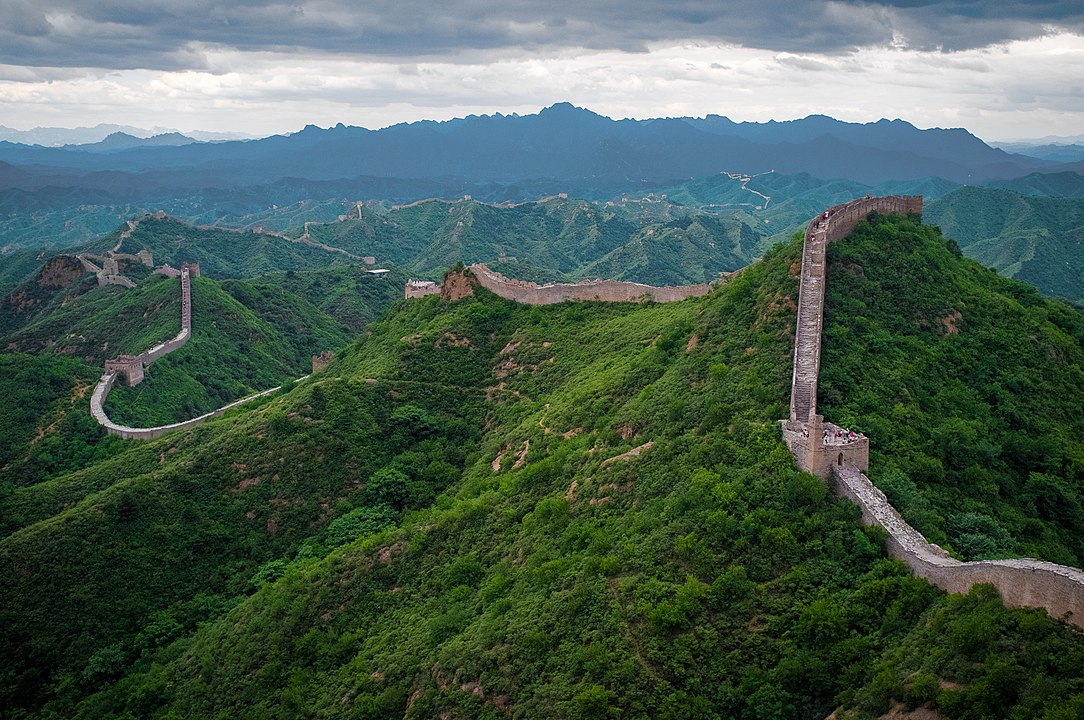
\includegraphics[width=\linewidth, keepaspectratio]{images/tgwoc.jpg}
							\caption{The great wall of China}
							\label{img:great-wall-of-china}
						\end{figure}
				\end{columns}
			}
			\only<4>{
				\begin{minipage}[t][0.3\textheight][t]{\textwidth}
					\begin{align*}
						i \hbar \frac{\partial}{\partial t} \Psi(\mathbf{r},t)=\hat H \Psi(\mathbf{r},t)
					\end{align*}
				\end{minipage}
				\begin{minipage}[t][0.7\textheight][t]{\textwidth}
					\small Lorem ipsum dolor sit amet, consectetuer adipiscing elit. Etiam lobortis facilisis sem. Nullam nec mi et neque pharetra sollicitudin. Praesent imperdiet mi nec ante. Donec ullamcorper, felis non sodales commodo, lectus velit ultrices augue, a dignissim nibh lectus placerat pede. Vivamus nunc nunc, molestie ut, ultricies vel, semper in, velit. Ut porttitor. Praesent in sapien. Lorem ipsum dolor sit amet, consectetuer adipiscing elit. Duis fringilla tristique neque. Sed interdum libero ut metus. Pellentesque placerat. Nam rutrum augue a leo. Morbi sed elit sit amet ante lobortis sollicitudin. Praesent blandit blandit mauris.
				\end{minipage}
			}
		\end{frame}
	\section{Overlays}
	\section{Themes}
\end{document}
